\chapter{Method}
\label{ch:method}

The transformer model has shown great potential on a variety of challenging \gls{nlp} tasks. Initially, the transformer was created to perform machine translation where it outperformed previous models by a vast margin~\cite{Vaswani2017}. In fact, at the time of writing, the transformer is the core of the Google translate engine.
\medskip

OpenAI uses the transformer to perform various \gls{nlp} tasks~\cite{Radford2018}. Their \gls{gpt}-model solves classification, entailment, similarity and multiple choice question answering tasks. They use a transformer encoder stack with 12 encoder blocks and task-dependent classification heads. 

They show that even though they use the same base transformer model for each task they achieve \gls{sota} results for most of the tasks.
\medskip

One year later, in 2019, OpenAI published \gls{gpt}-2 which is an extension to \gls{gpt}~\cite{Radford2019}. With \gls{gpt}-2 Radford et al. are able to achieve revolutionary results generating text with a transformer architecture\footnote{OpenAI does not plan to release the trained model for the language generation task as they are afraid that it will be used for malicious intents -- Source: OpenAI blog \url{https://openai.com/blog/better-language-models/}}. Again, they also achieve \gls{sota} results on other \gls{nlp} task mentioned above.
\bigskip

We propose the \acrfull{absat} which builds on the knowledge that the transformer is a powerful architecture useful for a variety of NLP tasks. Radford et al. already show that the transformer can be used to predict sentiment for a document~\cite{Radford2018}. 

However, sentiment analysis is one of the few tasks where \gls{gpt}-1 is not able to achieve \gls{sota} results. Moreover, \gls{gpt}-1 only classifies standard sentiment and not aspect-based sentiment.
\medskip

Our model is the first architecture which uses a transformer to perform multi-task aspect-based sentiment analysis. The next section describes the architecture of the \gls{absat} model. Section~\ref{sec:04_multitask} describes how \gls{absat} is used in combination with multi-task learning and finally, Section~\ref{sec:04_transferLearning} explains how we used transfer learning to boost the training performance.

\section{General Model Architecture}

The following section describes the proposed \acrfull{absat} architecture. As the name suggests, this design is based on the transformer model~\cite{Vaswani2017}. The second model characteristic is influenced by the work of Schmitt et al. and their concept of separate aspect heads for sentiment classification~\cite{Schmitt2018}.
\bigskip

\begin{figure}[htp]
    \centering
    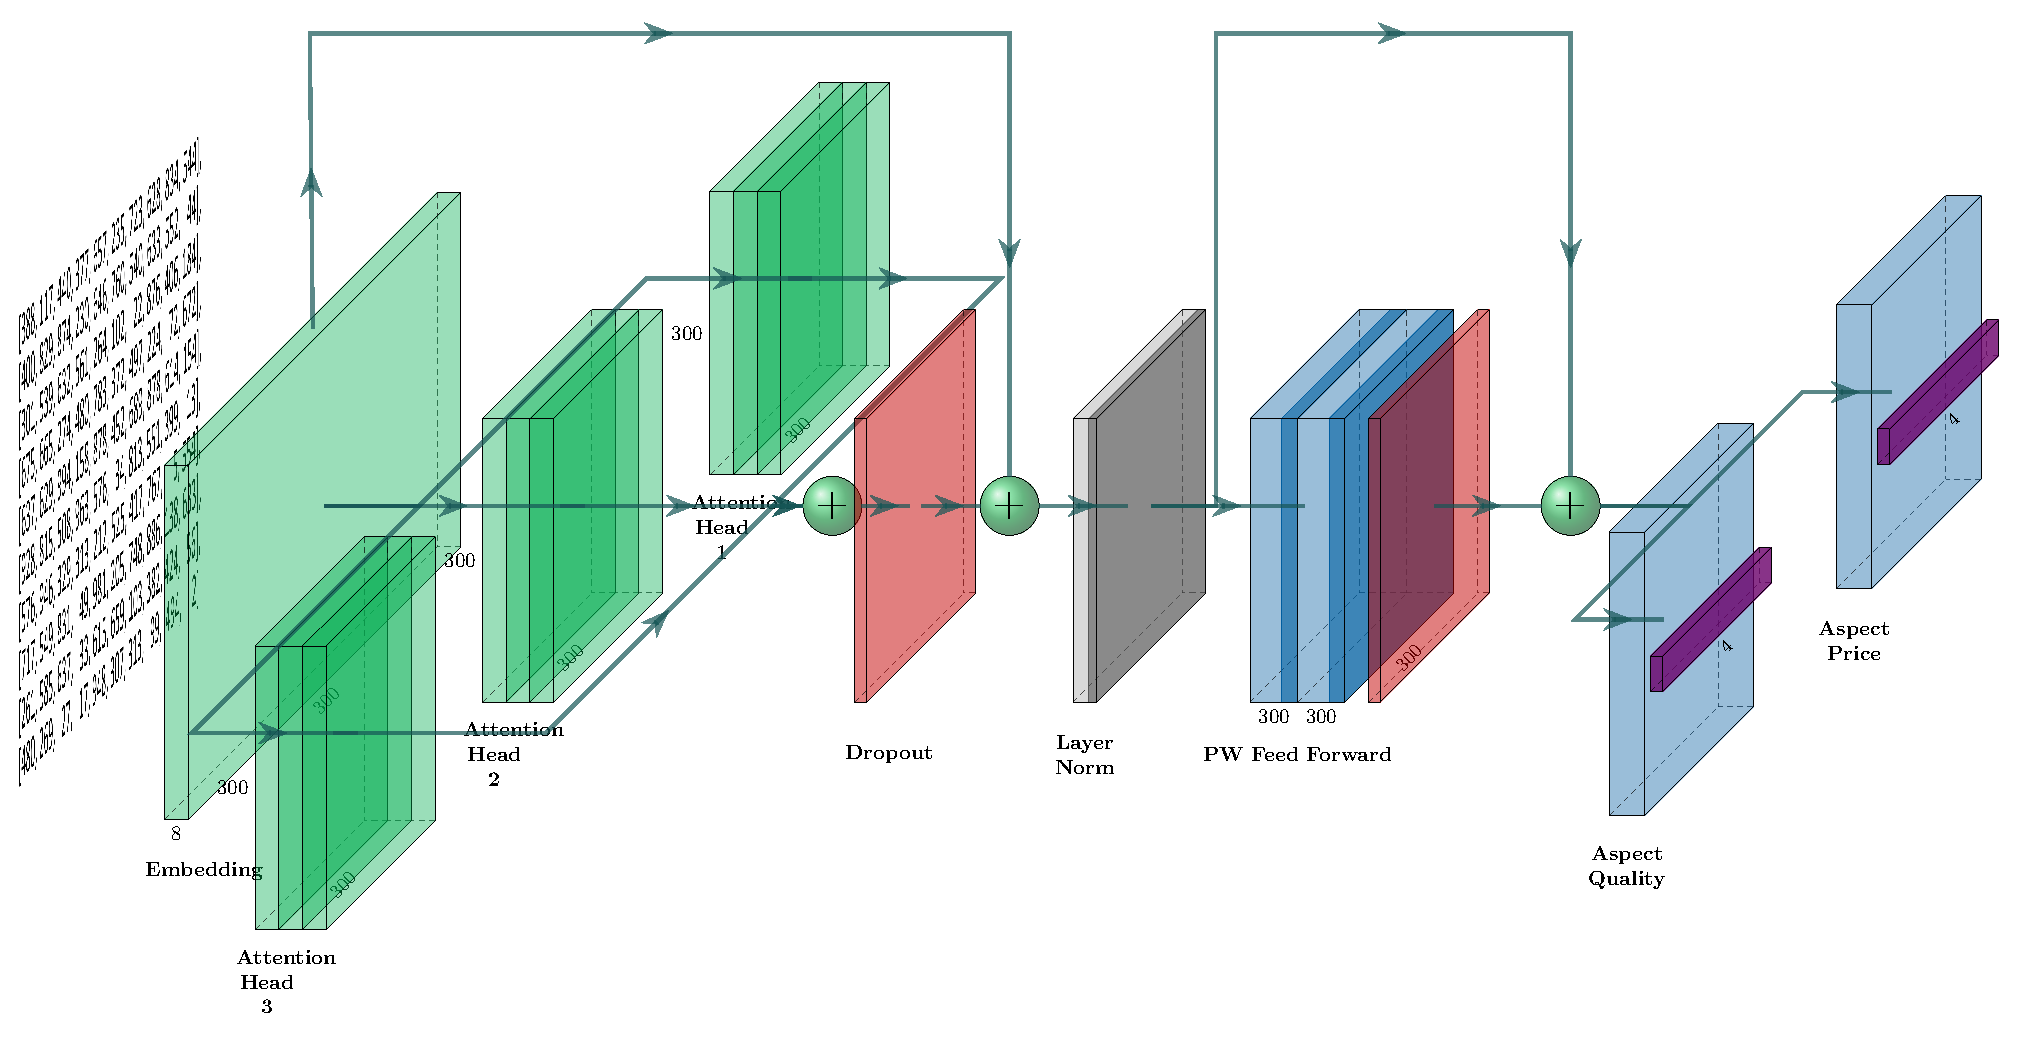
\includegraphics[width=\textwidth]{figures/04_method/04_t-absa}
    \caption{\textbf{Visualization of an exemplary \acrfull{absat} model} with one encoder block consisting of three attention heads and four aspect heads. The positional encoding is not visualized in this figure.}
    \label{fig:04_t-absa}
\end{figure}

Figure~\ref{fig:04_t-absa} visualizes a simplified \gls{absat} model. This specific instance consists one encoder block which contains 3 attention heads. To the right of the encoder block are four aspect heads. Each aspect head is trained to classify the sentiment for one aspect. In figure~\ref{fig:04_t-absa} those aspects are \textit{GMOs}, \textit{Quality}, \textit{Price} and \textit{Taste}. Each aspect has four output classes {(visualized in the figure for the "Pesticides"-aspect)}:

\begin{itemize}
    \item negative
    \item neutral
    \item positive
    \item not applicable {(N/A)}
\end{itemize}

Each aspect head is isolated from the rest which allows the transformer to perform multi-label \gls{absa}. When a document or sentence contains a specific aspect the corresponding aspect head outputs either \textit{negative}, \textit{neutral} or \textit{positive}. If this aspect is not part of the sentence, the output is \textit{not applicable}.

We propose two different versions of aspect heads which we describe in Section~\ref{sec:04_aspectHeads} in detail.

\section{Transformer}
\label{sec:04_transformer}

The original transformer uses undisclosed word embeddings which output a 512-dimensional vector\footnote{They also experiment with 256 and 1024 dimensional vectors}. It is possible that the original transformer does not use pre-trained embeddings. We performed experiments with \gls{absat} and untrained word embeddings but concluded that pre-trained word embeddings outperform untrained word embeddings. 

However, the difference was only a few percents, and it is conceivable that a transformer with more training data would be able to train its own word embeddings.
\medskip

Considering the smaller datasets that we use for \gls{absa}, the \gls{absat} model uses pre-trained embeddings instead of untrained embeddings. Pre-trained embeddings for both \gls{glove} and fastText are only available for up to 300 dimensions. As a consequence, the model size of our transformer is only 300 instead of 512.
\bigskip

Similar to the vanilla transformer, \gls{absat} also uses a \gls{adam} optimizer~\cite{Kingma2014} and a special learning rate decay which is called noam\footnote{It is not apparent what noam stands for or where this learning rate decay schema came from. It is not mentioned or cited as noam, but it is referred to as noam by the authors in discussions: \url{https://github.com/tensorflow/tensor2tensor/issues/280}}~\cite{Vaswani2017}

\begin{equation}
    \text{NOAM:} \quad lr = d_\text{model}^{0.5} * min(step\_num^{0.5}, step\_num*warmup\_steps^{-1.5})
\end{equation}
 
Contrary to the transformer model, we do not use label smoothing as a regularization technique. Experiments showed that this impacted the F1-score negatively. Instead, \gls{absat} uses weight decay with a decay value of $\epsilon_w = 1e-8$.


\section{Aspect Heads}
\label{sec:04_aspectHeads}

The transformer is designed as an encoder-decoder architecture with multiple stacks of encoders and decoders. Therefore, the input of an encoder {(or decoder)} has the same dimensionality as the output. Consequently, the input of an aspect head has the following dimensionality: $[batch\_size, s, d_{model}]$ where $d_{model}$ is the model size and $s$ is the sequence length. In other words, the transformer provides a $d_{model}$ dimensional vector for each word $w_i$ in a sequence.
\medskip

The aspect heads have the role of transforming this vector to a vector which can be used for sentiment classification. For aspect-based sentiment classification this dimension is $[batch\_size, 4]$.

\subsection{\acrfull{mlsa}}

\begin{figure}[htp]
    \centering
    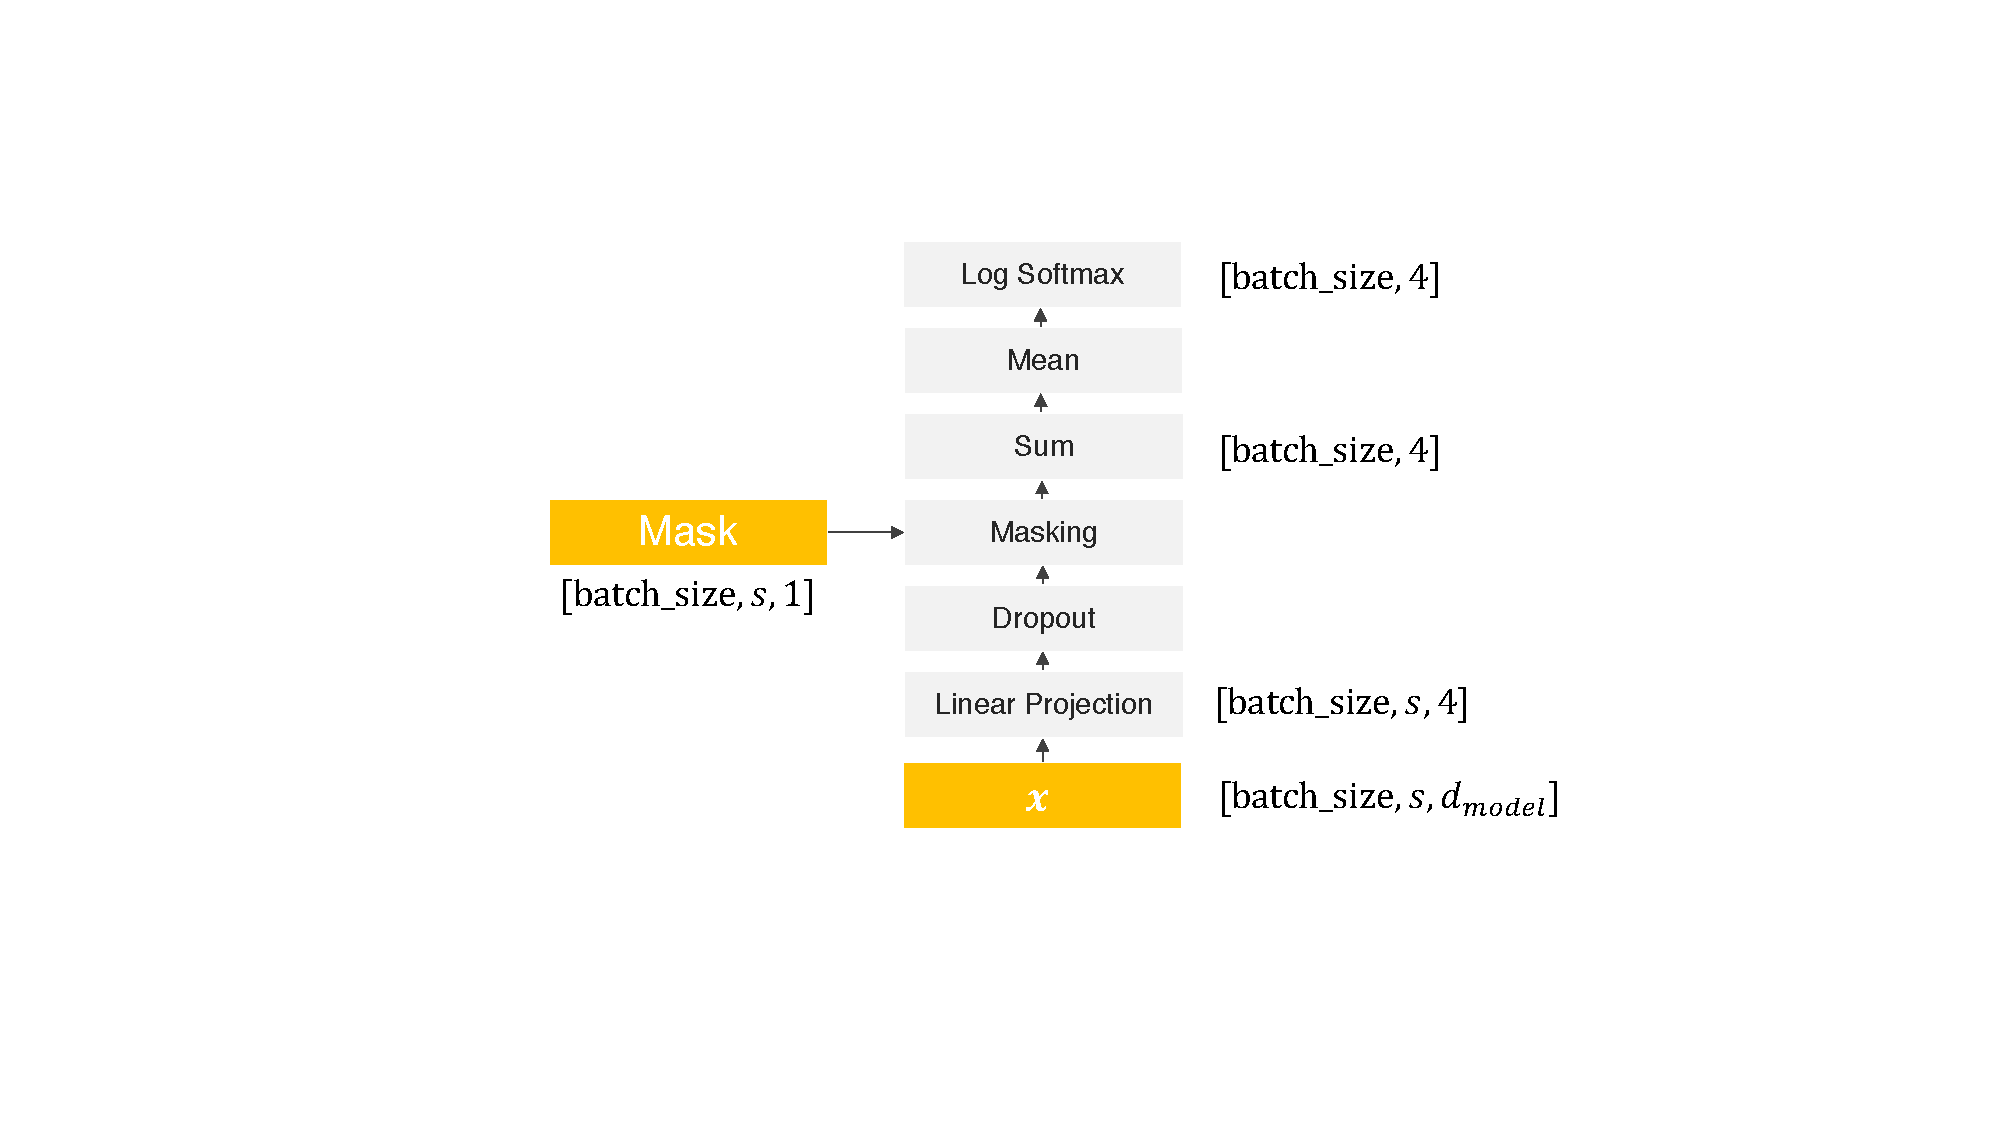
\includegraphics[width=0.7\textwidth]{figures/04_method/04_lmh}
    \caption{Visualization of the operations of an \gls{absa} \acrfull{mlsa}}
    \label{fig:04_lmh}
\end{figure}

The first aspect head design is called \acrfull{mlsa}. This head design consists of a linear layer which projects the $d_{model}$ dimensional word vector to a 4-dimensional word vector. This projection reduces the tensor to $[batch\_size, sequence\_lenght, 4]$. The tensor is then summed up along the second dimension, and the mean is taken. Finally, a softmax operation calculates the log probabilities.

Similar to the transformer layers, optional masking is applied on the tensor. Zeros replace predictions for words in the sequence which are only padding tokens.

\subsubsection*{Mean Operation}

The mean after the sum acts as a normalization for the prediction values before they pass through the softmax. The log softmax is defined as 

\begin{equation}
    \sigma(y_i)=log(\frac{e^{y_i}}{\sum_{j=1}^{K}e^{y_j}})\quad .
\end{equation}

As a consequence, large values for $y_{ij}$ result in very large negative values after the log softmax. This has two effects on the \gls{nll}-loss:

\begin{enumerate}
    \item Long sequences get a larger loss than shorter sequences. The reason for this is that the sum-function will sum up all predictions for every word in a sequence. Of course, a longer sentence will have a larger sum as they have more values to sum up. Therefore, the result of the softmax will be more negative which results in a higher loss.
    \item It is not possible to compare the loss of \glspl{mlsa} and \glspl{cnna}. \gls{cnna} uses a combination of convolutions and max pooling. Therefore, the numerical value of a prediction before the log softmax will usually be lower than for \glspl{mlsa}, since max pooling takes the maximum and not the sum.
\end{enumerate}

By using a mean operation before the log softmax, we can solve both problems.

\subsection{\acrfull{cnna}}
The \acrfull{cnna} uses convolutions in combination with max pooling to perform the final prediction. Figure~\ref{fig:04_ch1} visualizes the operations and how the tensor size changes during a forward pass through the head. 
\medskip
\begin{figure}[htp]
    \centering
    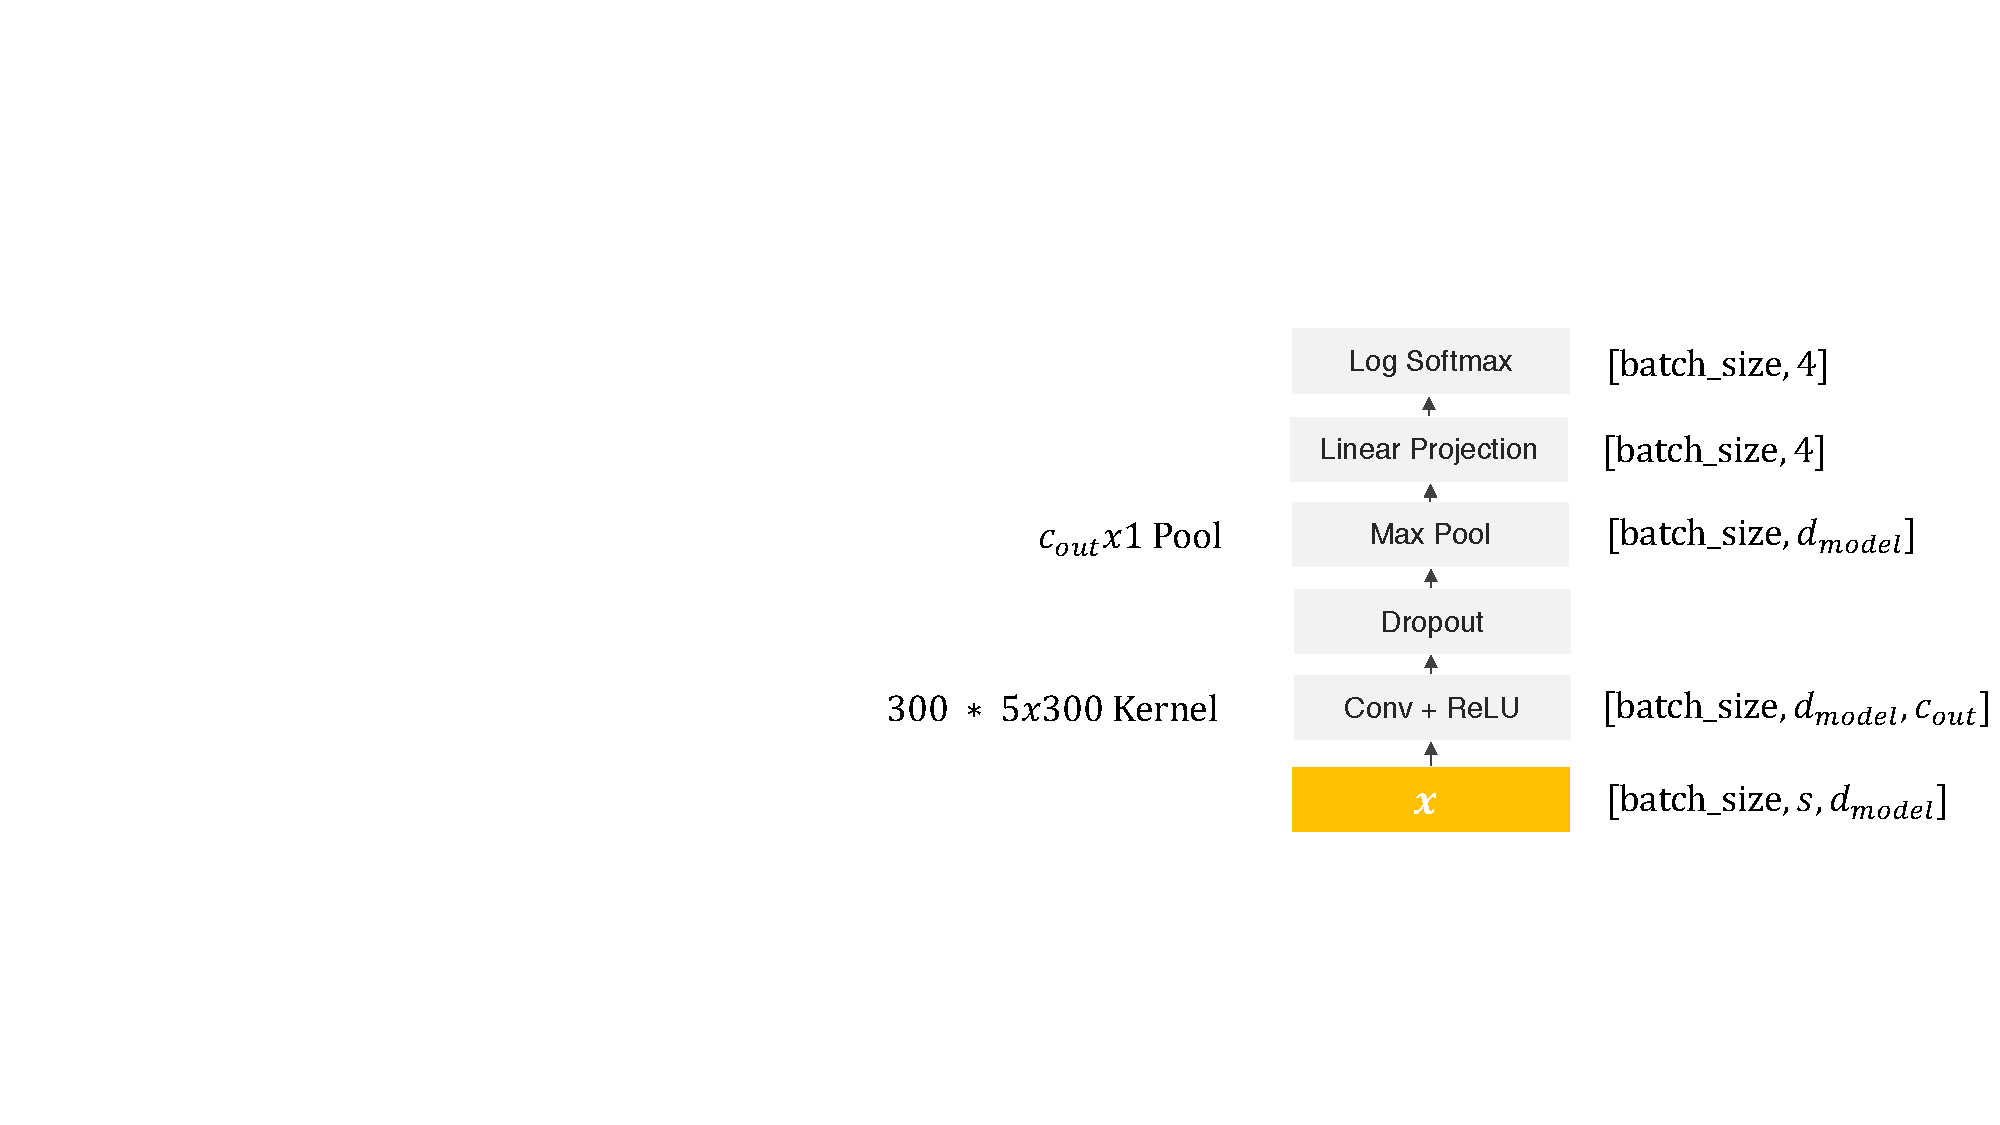
\includegraphics[width=0.7\textwidth]{figures/04_method/04_ch}
    \caption{Visualization of the operations of an exemplary \gls{absa} \acrfull{cnna}. This specific head uses a kernel size of 5 and 300 filters.}
    \label{fig:04_ch1}
\end{figure}

First, the tensor is passed through a convolutional layer. The filter size, the number of filters, stride, and padding, are controlled through hyperparameters. This means the size of subsequent layers depends on these parameters. The output size $c_{out}$ of the convolutional layer is given as:

\begin{equation}
    c_{out} = \frac{s+2*P-F}{S} + 1
\end{equation}

where $F$ is the filter size, $S$ is the stride, and $P$ is the padding amount. The max pooling layer reduces the tensor from $[.., d_{model}, c_{out}]$ to $[.., d_{model}]$ along the first dimension. Finally, a linear layer projects the output to class predictions and the log softmax scales the values.
\medskip

\begin{figure}[htp]
    \centering
    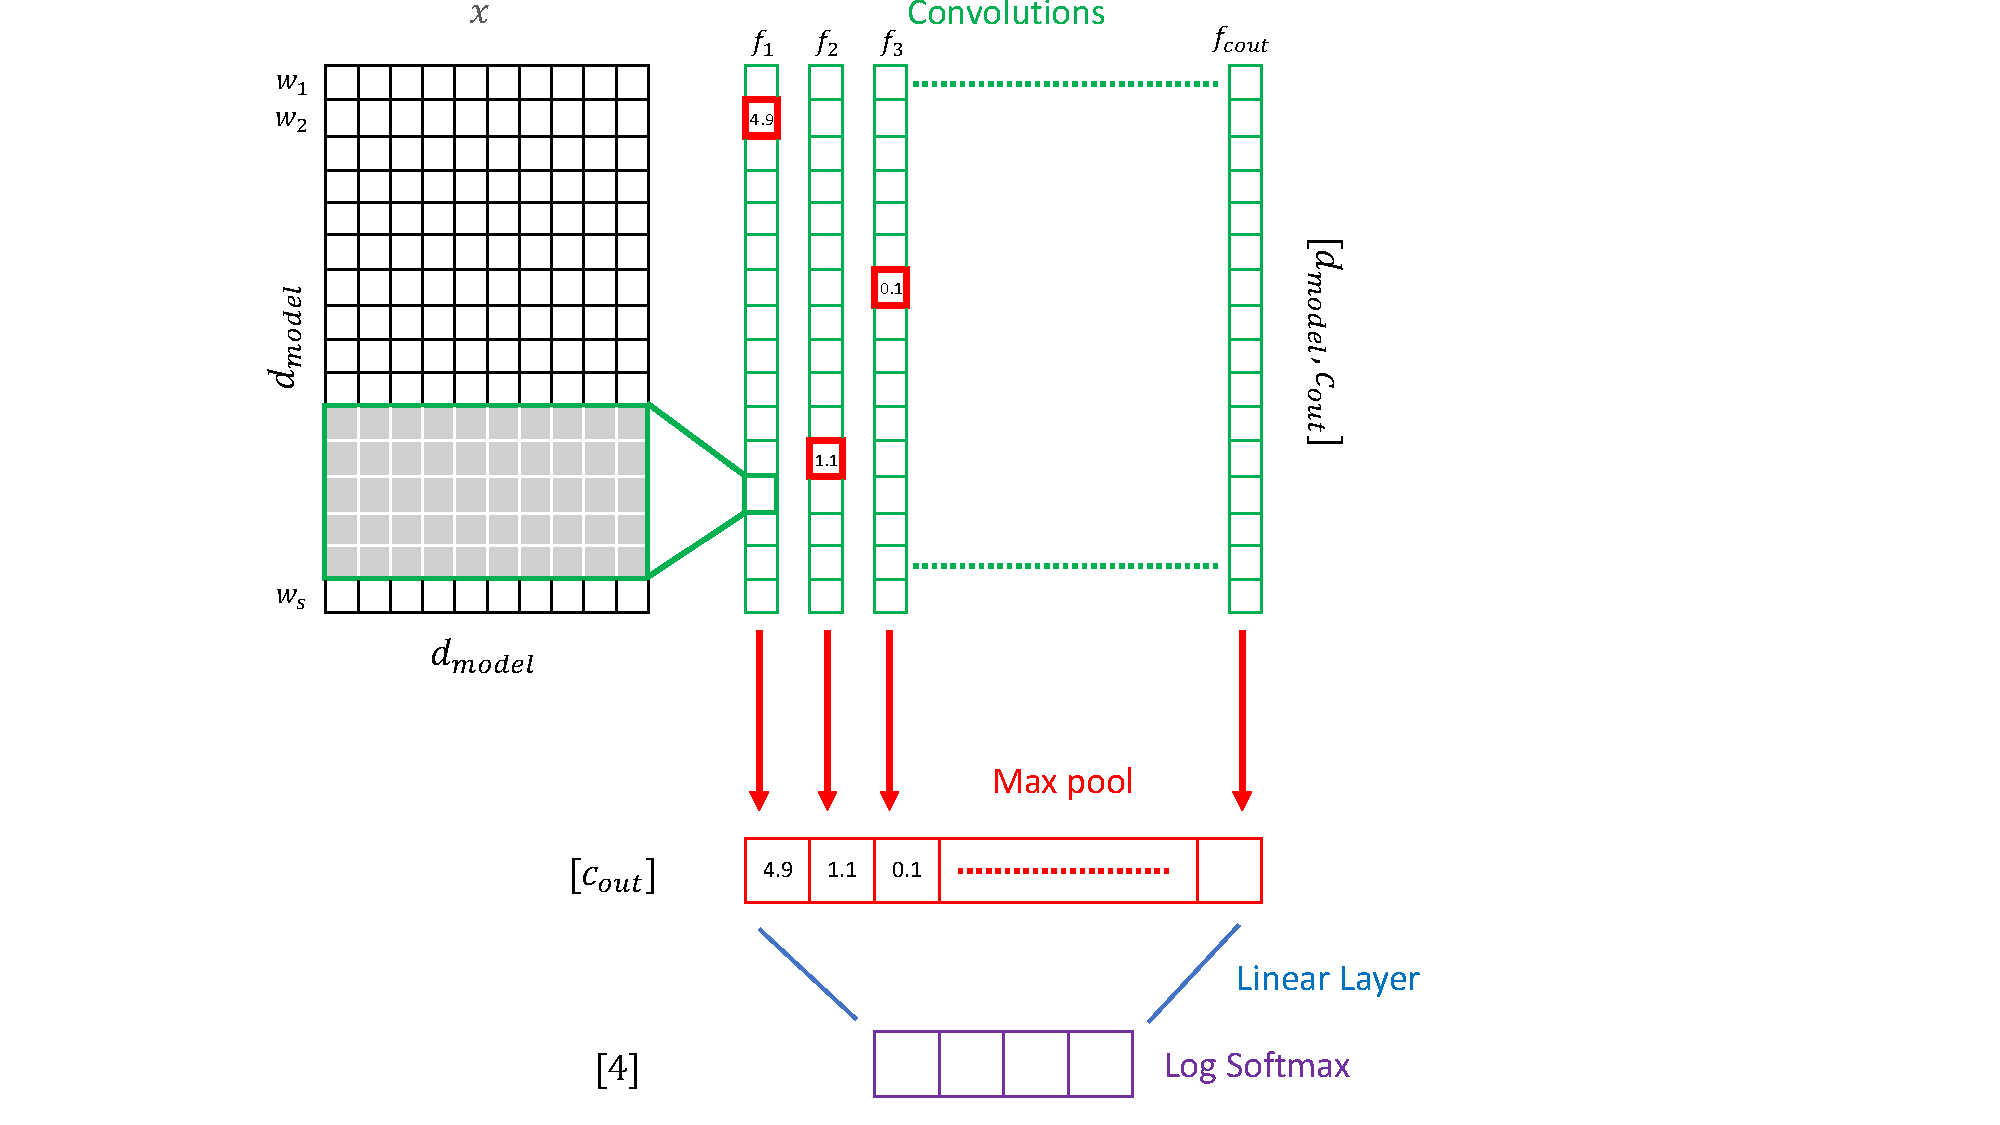
\includegraphics[width=0.7\textwidth]{figures/04_method/04_ch2}
    \caption{Visualization of the convolutional and max pooling operations of an \gls{absat} \gls{cnna} in detail. $w_1$ to $w_s$ are the words in a sequence with length $s$. This figure does not include the batch size as an extra dimension.}
    \label{fig:04_ch2}
\end{figure}

Figure~\ref{fig:04_ch2} depicts the convolution and the pooling in more detail.

\subsection{Weighted Loss}

Each aspect head calculates its own loss value using the predictions for the aspect as the targets. To combat data imbalance, we use a weighted NLL loss which is given as

\begin{equation}
\mathcal{L}_\text{NLL}=-\frac{1}{n}\sum_{i=1}^{n} w_i * (y_i \cdot log(\hat{y}_i))
\label{eq:04_nll}
\end{equation}

where $n$ is the number of classes, $w_i$ is the specific class weight, $y_i$ is the ground truth and $\hat{y}_i$ is the prediction. Since we only use the aspect heads for sentiment classification, $i$ will always be either a sentiment or not applicable. Therefore $i \in \{\text{negative}, \text{neutral}, \text{positive}, \text{not applicable\}}$ and $n=4$.
\medskip

The class weights are calculated during data loading. The equation for the calculation of a weighted scalar for a class weight for class $i$ is given as

\begin{equation}
    w_i = 1 - \frac{x_i}{N}
\label{eq:04_cls_weight}
\end{equation}

where $x_i$ is the sum of all of $i$-s occurrences for the aspect. $N$ is the total number of times an aspect occurred in the dataset.
\medskip

Equation~\ref{eq:04_cls_weight} assigns a low numerical value to classes which occur more frequently. As a consequence, the \gls{nll}-loss is lower for frequent classes with low-class weights which reduces the influence of those common classes.  

\section{Multi-Task Learning}
\label{sec:04_multitask}
The way the \gls{absa}-Transformer is build, inevitably necessitates multi-task learning since for each aspect-head a separate \gls{nll}-loss is computed. For each of the $m$ aspect classes a loss value is calculated. In the end the mean of all losses is taken as shown in equation~\ref{eq:04_multiheadLoss}:

\begin{equation}
\mathcal{L}_\text{MultiTask} = \frac{1}{m}\sum_{j=1}^{m}\mathcal{L}(f(x), y_m)
\label{eq:04_multiheadLoss}
\end{equation}

where $\mathcal{L}(f(x), y_m)$ is the \gls{nll}-loss of the model $f$ with input the $x$ defined in equation~\ref{eq:04_nll}.

\subsection{Multitask Task Data Augmentation}

As described in Section~\ref{sec:03_mtlAdvantages} it is also possible to augment the data by using an auxiliary task in addition to the regular classification tasks.
There are three possible auxiliary tasks to consider:


\begin{enumerate}
    \item Predict an additional label from the source data
    \item Use an additional dataset B in combination with the source dataset A and predict labels for the classes in A and the classes in B simultaneously. This approach is similar to transfer learning, but instead of training the models sequentially, this approach would train them together.
    \item Predict additional aspects of the source data which can be trained unsupervised.
\end{enumerate}

This thesis focuses on the first type of auxiliary task where we try to predict a new label for the source dataset. As the source dataset, we choose the GermEval-2017 dataset since this dataset provides an additional document-wide sentiment label. This label was chosen since the other aspect heads already perform sentiment analysis so this task is very similar on the one hand. On the other hand it can provide additional data points for the training of the model. In addition, the dataset provides a reasonable amount of training data.

Training with the auxiliary sentiment label is performed by adding an additional sentiment head to the model. During training the loss of the auxiliary tasks contributes to the improvement of the transformer base.

However, during evaluation, this task is ignored when calculating the F1-score for the model.
\medskip

The results for this experiment is located in Section~\ref{sec:06_ResultsMultitask}.

%We also experiment with the weighting of the tasks in the loss


\section{Transfer Learning}
\label{sec:04_transferLearning}

Besides, multi-task learning we also perform transfer learning to test if the transformer can transfer knowledge from one domain to another domain. The transformer model is often used for language modeling and language understanding. These tasks are essential for every \gls{nlp} task in general and sentiment analysis specifically. Hence, the transformer base should be domain independent. 
\medskip

It has been already shown that transferring knowledge from the word embedding layer from one domain to another is not only possible but beneficial for the overall performance~\cite{Yosinski2014}. Therefore, in addition to the transformer base, we also use pre-trained word embeddings.
\medskip

Due to the nature of the aspect heads, we can not transfer knowledge from one domain to another. Not only are aspect heads highly domain specific but also aspect specific. 
\smallskip

We performed experiments to test this theory. To do this, we trained the model on a dataset, stopped training and then reshuffled the aspect heads so that they would need to predict different aspects from there on. 

This experiment was performed to answer two questions: 

\begin{enumerate}
    \item How much predictive power originates from the transformer and how much is produced by the aspect heads in comparison.
    \item Is it possible to transfer knowledge from aspect heads to a different domain?
\end{enumerate}

In other words, this was a transfer learning experiment on the same dataset.

The results were in line with our theories that the transformer produces the majority of the domain independent knowledge. After the training was stopped and the aspects were reshuffled, the evaluation score dropped back to a level which would usually be achieved after the first or second epoch. Of course, this experiment did not improve upon the final F1 score of the model. After a few epochs, the evaluation score was back to the levels were training was previously stopped. This being said, the number of iterations it took to reach that score was shorter than on the first run.
\medskip

\subsection{Knowledge Transfer from Amazon Reviews}

In Section~\ref{sec:06_ResultsTransfer} we perform experiments to asses the theory about the transferability of the transformer base. We train a transformer model on the Amazon reviews dataset {(Section~\ref{sec:05_amazonReviews})} which we collected just for this experiment. This dataset is very large and balanced along the aspect dimension.
\medskip

After the transformer completes training, we take the models embedding and transformer base and exchange the aspect heads with new heads for the training on the target dataset. For the target dataset we use  the organic-2019 dataset {(Section~\ref{sec:05_organic2019})}.
\bigskip

\subsubsection*{Transfer of Knowledge from Word Embeddings}

Word embeddings encode vast amounts of information. In fact it makes up a majority of the trainable network parameters {(see Section~\ref{sec:06_ResultsAmazon})}. Furthermore, the transformer is conditioned on the word vectors the embedding produces as they shift from the pre-trained embeddings to more domain specific embeddings. This can be observed when we freeze the embeddings during training so that they do not change. This freezing significantly impacts the performance negatively.
\medskip

Unfortunately, this is a threat to the transferability of the embedding layer. When the embeddings are first created, they are initialized with the vocabulary of the dataset. Especially, for the amazon dataset, there is a considerable number of infrequent words {(see Section~\ref{sec:05_amazonTokens})} that do not necessarily occur in the target dataset. Even when removing the most infrequent tokens a large percentage of the vocabulary from the amazon dataset is not used for the target dataset which makes a large portion of the embedding domain specific. 
\medskip

On the other hand, there are tokens in the target dataset which do not occur in the Amazon reviews dataset. For the organic dataset, these tokens are highly domain specific. Most of these tokens are chemical compounds and other words like "Glyphosate" which are very important for this dataset.
\medskip

To solve this dilemma we combine both vocabularies before we start with the training on the amazon dataset. By doing this, we ensure that both tasks can use the same embedding layer. 

Unfortunately, due to computational restraints on the \gls{gpu} memory, we have to restrict the size of the shared vocabulary further. This restriction implies that we can not create embeddings for every token in the dataset and some infrequent tokens have to be replaced with \textit{<UNK>}.
\medskip

For this reason, we cannot compare the results of the transfer learning experiments directly with the best results on the individual datasets. However, we perform a baseline run with the same vocabulary restrictions so that we can asses the effect of the transfer learning experiment.